\chapter{Trabalhos relacionados}

Após uma busca pela literatura, foi encontrada uma tese de doutorado escrita por \citeonline{Thesis:2019}, intitulada ``\textit{Learning Analytics Integrating Student Attendance Data}'', é uma pesquisa que explora a aplicação de técnicas de análise de dados para melhorar a compreensão do comportamento dos alunos em relação à frequência às aulas. A tese examina como os dados de frequência podem ser coletados, analisados e usados para melhorar o desempenho acadêmico dos alunos. A tese argumenta que a análise dos dados de frequência pode fornecer informações valiosas sobre o comportamento dos alunos e ajudar a identificar padrões que possam ser usados para melhorar o desempenho acadêmico, e apresenta um estudo empírico que usa técnicas de aprendizado de máquina para analisar os dados de frequência dos alunos, mostrando ser possível prever com precisão o desempenho acadêmico dos alunos com base em seus padrões de frequência às aulas.

Durante o trabalho, a autora utilizou a metodologia de ``\textit{data-first}'', abordagem que prioriza os dados como o ponto central em todo o processo de tomada de decisões e desenvolvimento de estratégias, para isolar e explicar a discrepância nos dados de frequência dos alunos. Em vez de tentar encontrar um evento conhecido no conjunto de dados, ela tentou identificar eventos candidatos dentro dos dados e, em seguida, explicá-los como uma atividade secundária. Essa abordagem permitiu que ela explorasse os padrões de frequência dos alunos e identificasse possíveis eventos que poderiam estar afetando a frequência. A metodologia utilizada pela autora baseou-se nos resultados do modelo preditivo. Ela usou esses resultados para responder à seguinte pergunta de pesquisa:  ``Esse modelo pode ser usado para fornecer informações adicionais sobre os padrões de frequência dos alunos?'', identificando métodos e ferramentas apropriados para análise numérica e estatística. Cada candidato precisava ser correlacionado com um evento acadêmico, social ou físico. Para realizar sua pesquisa, a autora utilizou uma abordagem mista que combinava métodos quantitativos e qualitativos, coletando dados quantitativos sobre a frequência dos alunos usando o sistema de gerenciamento de aprendizagem da universidade. Também utilizou técnicas estatísticas avançadas para analisar os dados coletados. Ela usou análise descritiva para descrever as características básicas dos dados, como média, mediana e desvio padrão, e também uma análise multivariada para examinar as relações entre as variáveis e identificar possíveis padrões.

A autora realizou uma vasta revisão da literatura em várias áreas, incluindo ciência da computação, ciência de dados, psicologia, filosofia moral e educação. Essa revisão permitiu que a autora identificasse as melhores práticas e tendências atuais em análise de dados educacionais. Durante a tesa foi investigado separadamente cada uma das ferramentas/ambientes/sistemas mais populares ou mais citados usando fontes como publicações acadêmicas, folhetos de dados públicos ou literatura de produtos/demonstrações, o que permitiu que ela avaliasse as diferentes ferramentas disponíveis para análise de dados educacionais e determinasse quais seriam mais adequadas para sua pesquisa. No entanto, é importante notar que essas fontes não produzem uma avaliação completa em todas as situações, e a autora reconhece que essas fontes podem não fornecer uma avaliação completa das ferramentas em todas as situações e que pode haver outras ferramentas disponíveis que não foram incluídas em sua pesquisa.

Ao utilizar um modelo de aprendizado de máquina para identificar alunos que estavam em risco de se tornarem desengajados e faltosos e comparando os resultados do modelo com o método anteriormente utilizado pela universidade, a autora descobriu que o modelo de aprendizado de máquina identificou 62 alunos que não foram identificados pelo método anterior. Adicionalmente, a autora descobriu que a métrica de engajamento comportamental (BEM) era mais poderosa do que uma simples razão de sessões frequentadas, observando melhoria empírica de 12\% usando a métrica BEM em comparação com a razão de engajamento (ER). No entanto, ela não forneceu análise numérica e teoria matemática para explicar por que isso pode ser verdade. Por fim, também foi descoberto um padrão de grandes variações na contagem de alunos acima e abaixo do valor médio BEM em cada semana entre as semanas 5 e 8 do primeiro semestre. Ela usou essa observação para tentar isolar possíveis causas ou explicações para o efeito da falta de engajamento dos alunos.

% escrever mais algumas páginas
% - como que fez, com que técnicas, metodologia, forma de avaliação, resultados
% - figuras e esquemas sempre bom

Há também a dissertação de \citeonline{moissa2016}, que teve como o objetivo geral avaliar a influência das ferramentas de LA na interação, desempenho e satisfação dos alunos em ambientes virtuais de aprendizagem. Para alcançar esse objetivo, a autora propõe a realização de um experimento com usuários reais, a análise dos dados coletados e a comparação entre os alunos que tiveram acesso à ferramenta e os alunos que não tiveram, bem como entre os alunos que usaram a ferramenta e os que não usaram. Ainda que a autora teve foco específico em ambiente educacionais virtuais, o trabalho possui semelhança com o atual por buscar entender como as ferramentas de LA podem ser utilizadas para melhorar a experiência de aprendizagem de estudantes, compreendendo a influência dessas ferramentas para ajudar a desenvolver estratégias mais eficazes de ensino.

Para realizar a coleta dos dados, a autora desenvolveu ferramentas para auxiliar no processo de ensino-aprendizagem e realizou um experimento com usuários reais. Através desse experimento, foram coletados dados sobre a interação dos alunos com a ferramenta, seu desempenho e sua satisfação. Os dados foram analisados através de técnicas estatísticas e de Mineração de Dados, como análise de regressão, análise de correlação e análise de \textit{cluster}. Além disso, a autora aplicou um questionário de satisfação para coletar a opinião dos alunos em relação ao minicurso realizado e à ferramenta utilizada, sendo o questionário composto por questões objetivas, questões discursivas e questões de múltipla escolha.

\section{Iniciativas no exterior}
\label{sec:exterior}

Estudos de ponta sobre sistemas de frequência escolar no exterior costumam ser realizados em países classificados como desenvolvidos, sempre com o objetivo de garantir que os estudantes estejam frequentando as aulas e participando ativamente das atividades escolares, o que contribui para uma educação de qualidade e para a promoção da igualdade de oportunidades na sociedade. Isso pode significar não apenas a detecção da frequência por si só, mas também como o aluno está se comportando dentro da sala de aula, ou seja, se está realmente presente.

Uma das tecnologias mais utilizadas em sistemas de frequência de ponta é a detecção facial, seja por fotos ou por vídeos. Neste contexto, dois trabalhos são apresentados. O primeiro, \cite{bhat:2020}, utilizou a tecnologia de \textit{Deep Learning} para a detecção facial em vídeos de até 33 \textit{frames per second} (fps). O sistema proposto foi desenvolvido com base em uma abordagem de aprendizado de máquina conhecida como \textit{One Shot Learning}, que envolve a capacidade de reconhecer objetos ou rostos com apenas uma única imagem de treinamento, o tornando capaz de identificar um grande número de alunos com apenas uma foto (\textit{frame}) de referência. A precisão do sistema é superior a 90\%, o que faz com que seja possível concluir que o sistema poderia ser útil para aplicação futura não apenas em escolas, mas também em empresas, possuindo baixo custo de implementação.

O segundo trabalho, de \citeonline{chauhan:2022}, implementou um sistema de frequência baseado em reconhecimento facial, utilizando uma metodologia baseada na combinação de Análise de Componentes Principais (PCA) com Redes Neurais Convolucionais (CNN). O sistema é capaz de realizar uma verificação cruzada entre a imagem capturada e as imagens do banco de dados, e registrar a frequência do estudante caso haja correspondência. Os dados são então salvos em uma planilha do \textit{Excel}.

Um outro trabalho apresenta uma maneira de detecção de frequências utilizando Internet das Coisas (IOT). \citeonline{fawaz:2019} teve como objetivo desenvolver um sistema de frequência baseado em \textit{Radio Frequency Identification} (RFID), ou Identificação de Rádio Frequência), com foco em segurança, portabilidade e prontidão para ser implantado em larga escala. O sistema fornece uma solução prática e eficiente para monitorar a frequência dos alunos, utilizando o sistema IoT para registrar e buscar dados em um servidor ou nuvem, tornando-os disponíveis para o usuário a qualquer momento e em qualquer lugar. O trabalho também propõe que os próprios alunos possam conferir os próprios dados a qualquer momento. O artigo de \citeonline{fawaz:2019} também utiliza de um sistema IoT, porém com a tecnologia \textit{Wireless Sensor Networks} (WSNs), cuja proposta era criar cadeiras inteligentes, equipadas com sensores de peso e amplificadores que enviam sinais digitais para um receptor, permitindo a identificação da presença dos alunos durante o horário de aula. Também foi instalado um leitor de impressões digitais para aumentar a segurança e identificação dos alunos.

Outra solução para o problema de detecção de presenças são os dispositivos vestíveis, cujo mapeamento sistemático da literatura de \citeonline{ferreira:2020} aponta bons estudos da área. Segundo os autores, os países que possuem estudos na área são Estados Unidos, França, Itália, China, Japão, Eslovênia e Reino Unidos, a maioria com crianças do ensino fundamental de entre 7 a 13 anos. O trabalho investigou o posicionamento dos sensores, a maneira de armazenamento de dados e a validação dos dados, trazendo à tona que alguns dos trabalhos também focavam em coletar dados sobre a saúde física dos estudantes. O trabalho também cita que nenhum estudo brasileiro foi encontrado, trazendo a hipótese de que a baixa qualidade da infraestrutura de muitos contextos educacionais brasileiros poderia ser um impeditivo desse tipo de estudo em território nacional. 

\section{Iniciativas no Brasil}
\label{sec:brasil}

A Base de Dados do Cadastro Único para Programas Sociais (CadUnico) é uma ferramenta utilizada pelo Governo Brasileiro para registrar informações sobre famílias em situação de vulnerabilidade social, além de ser uma importante fonte de dados sobre a escolaridade no Brasil, pois registra informações sobre a escolaridade dos membros das famílias cadastradas que são utilizadas para monitorar e avaliar as políticas públicas de educação, bem como para identificar as famílias que precisam de apoio para garantir o acesso e a permanência na escola \cite{garcia:2017}. Desde sua criação, a base de dados CadUnico tem recebido diversos prêmios, como o prêmio de Inovação na Gestão Pública Federal, concedido em 2017 pelo Ministério do Planejamento, Desenvolvimento e Gestão, e o Prêmio Excelência em Governo Eletrônico, concedido em 2016 pela Associação Brasileira de Entidades Estaduais de Tecnologia da Informação e Comunicação.

No que diz respeito à unificação da base de frequência com o chamado Sistema Presença, o Brasil tem buscado implementar medidas para garantir o registro da frequência escolar de todos os estudantes. O Sistema Presença foi lançado em 2019 pelo MEC com o objetivo de padronizar as informações sobre a frequência escolar em todo o país. Antes da criação do sistema, as informações sobre a frequência dos estudantes eram registradas em diferentes sistemas pelos estados e municípios, o que dificultava o acompanhamento e a análise dessas informações. Vale destacar que a chave única de identificação dos alunos neste sistema é o Número de Identificação Social (NIS), que é gerado pelo CadUnico. No entanto, a implementação do Sistema Presença tem enfrentado alguns desafios, como a necessidade de capacitação dos profissionais envolvidos no registro e análise dos dados, para responsáveis pela coleta e análise dessas informações estejam devidamente preparados para lidar com as novas tecnologias e sistemas de informação. Outro desafio é a questão de investimentos em infraestrutura tecnológica para garantir o funcionamento do sistema em todo o país, o que envolve desde a aquisição e manutenção de equipamentos e softwares até a disponibilidade de uma conexão de internet estável e rápida, especialmente em regiões mais remotas~\cite{echazarra2019learning}. Por fim, a pandemia de COVID-19 trouxe novos desafios para a implementação do sistema, especialmente no que diz respeito à adaptação do sistema às novas modalidades de ensino remoto. Com a suspensão das aulas presenciais em muitas regiões do país, foi necessário buscar alternativas para registrar a frequência dos estudantes em aulas virtuais e atividades remotas. Isso exigiu uma adaptação rápida do sistema e dos profissionais envolvidos, bem como investimentos adicionais em tecnologias e recursos para permitir a coleta dessas informações.

Com o Sistema Presença, o acompanhamento da frequência dos estudantes tornou-se mais efetivo, mesmo com os desafios de questões profissionais e monetárias, o que pode contribuir para a promoção de políticas públicas mais eficazes na área da educação. Em uma pesquisa realizada pelo MEC, em 2019, ano de implementação do sistema, a frequência escolar alcançou os melhores índices históricos, como é possível verificar pela Figura \ref{fig:my_label} \cite{historicos2019}. As duas imagens representam o histórico de frequência entre os anos de 2007 (um ano após a implementação do Sistema Presença) e 2019, indicando que houve índices recordes de frequência escolar em todo o país; ou seja, a taxa de alunos beneficiários dentro da sala de aula, entre fevereiro e março de 2019, chegou a 90,31\%, e entre abril e junho, em 89,81\%.

\begin{figure}[ht!]
    \centering
    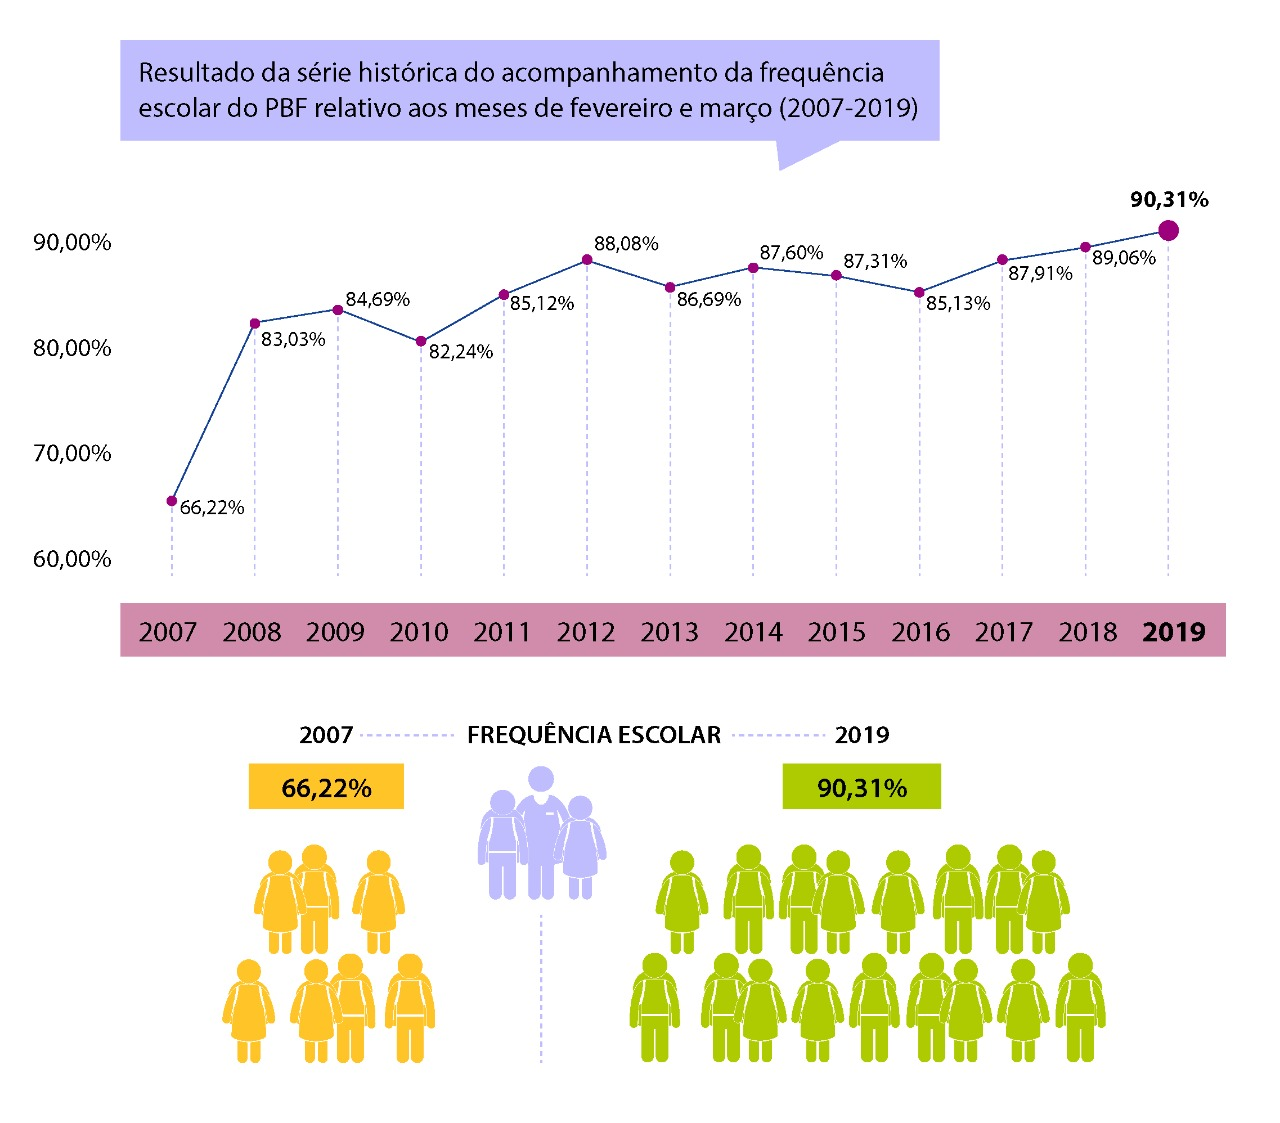
\includegraphics[width=0.46\linewidth]{Textuais/Imagens/image1.png}
    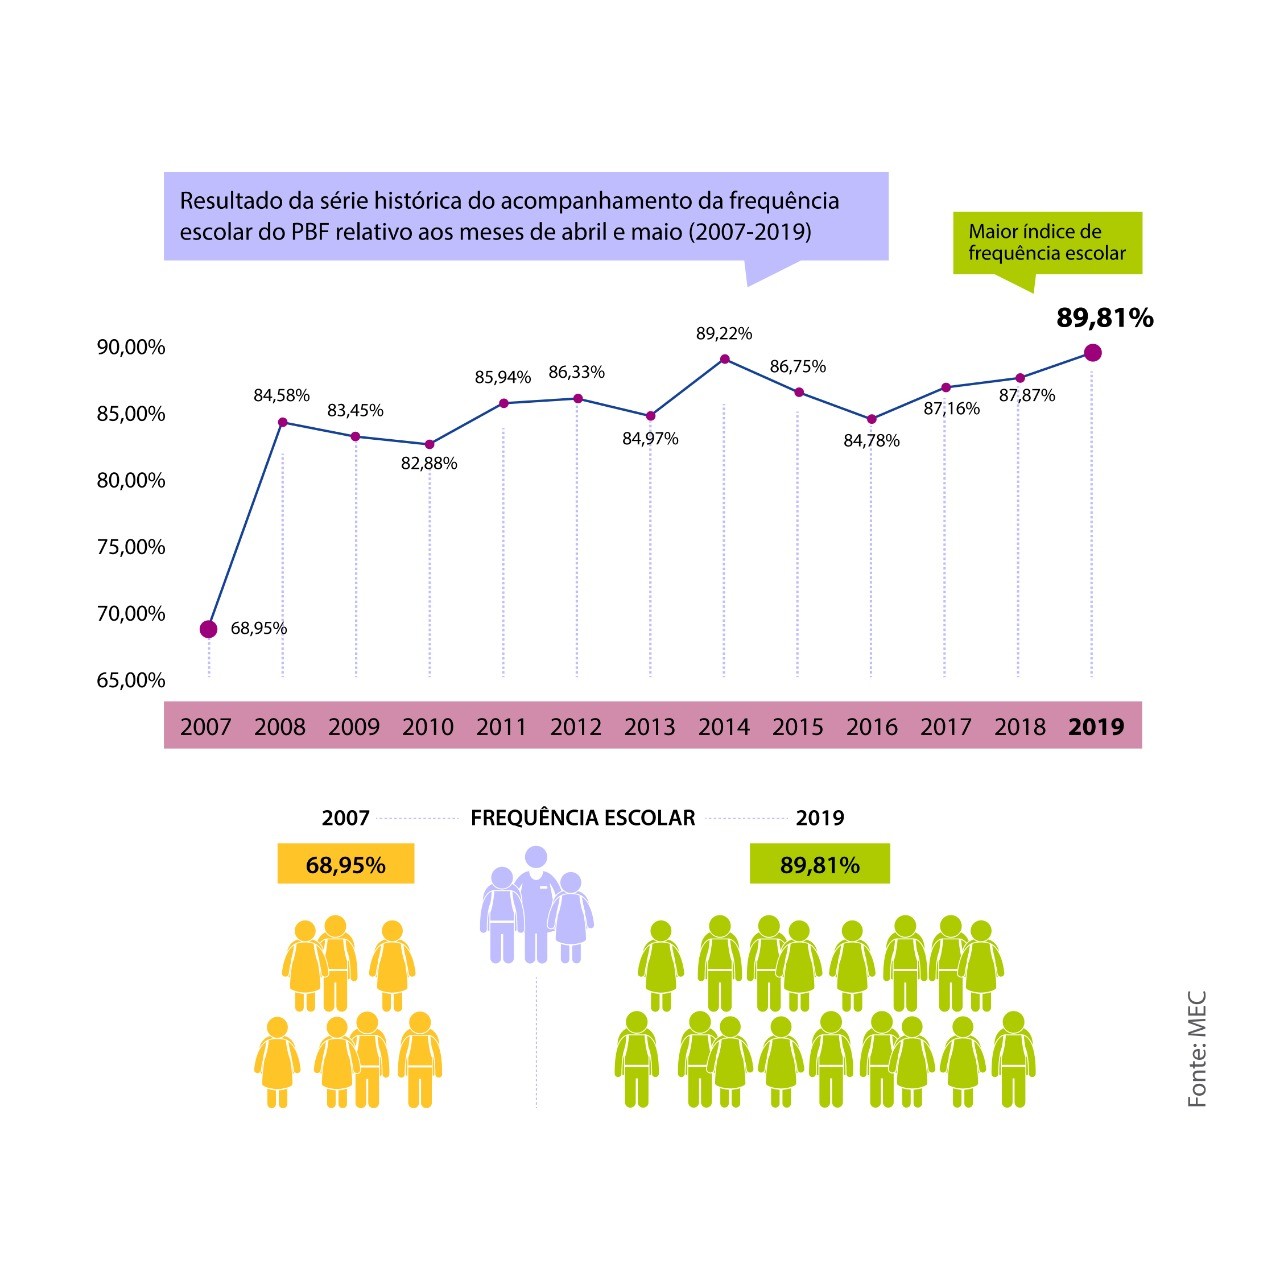
\includegraphics[width=0.46\linewidth]{Textuais/Imagens/image.png}
    \caption{Histórico de frequência de estudantes no Brasil entre os meses de fevereiro a março, e de março a abril de 2019.}
    \label{fig:my_label}
\end{figure}


O Sistema Presença tem limitações importantes. Como o objetivo deste sistema é fornecer dados para o Bolsa Família, apenas alunos beneficiários deste programa têm sua frequência coletada. Além disso, a frequência é coletada com granularidade mensal. Isto impossibilita o desenvolvimento de ferramentas de alerta de evasão, baseadas em Inteligência Artificial, que sejam capazes de detectar padrões nos dados e permitam ações de combate à evasão em um estágio precoce. Por outro lado, não há a integração dos dados de frequência com outros dados relevantes do estudante, como dados de desempenho escolar. Embora o Sistema Presença ainda esteja em fase de implementação, desde o início dos anos 2000 houveram estudos foram conduzidos com o objetivo de resolver o problema de coleta de dados de frequência de forma mais eficiente \cite{Soligo_2010}. É o caso do trabalho de \citeonline{pereira:2012}, que apresenta uma proposta de monitoramento do estudante no momento de chegada e saída da instituição, sendo realizada em tempo real a comunicação aos responsáveis através do envio de SMS. Adicionalmente, será possível a geração de relatórios acerca da frequência escolar do aluno. A utilização da aplicação proposta visa tornar o controle de frequência mais rápido e eficiente, além de proporcionar a comunicação dos dados coletados aos responsáveis do discente, estabelecendo a sensação de segurança por parte da instituição. Além da frequência, há dispositivos que buscam coletar outros tipos de dados de alunos em sala de aula, como demonstrado no projeto de \citeonline{ferreira:2022}. Neste projeto, foram utilizados objetos vestíveis para detectar os movimentos das crianças do ensino fundamental, a fim de observar o comportamento dos alunos em sala de aula e compreender melhor a rotina escolar. A metodologia utilizada para coletar os dados de movimento das crianças foi a utilização de um dispositivo \textit{wearable Actigraph GT9X Link}, que possui dois acelerômetros e um giroscópio, sendo estes os sensores de captação de movimento. As informações geradas tratam-se de registros em arquivo dos pontos dos eixos de (x, y, z) de cada um dos sensores para cada centésimo de segundo. Para ser traçado o perfil dos estudantes voluntários, foram enviados formulários aos responsáveis que envolviam perguntas como idade, peso, altura, sexo, mão com a qual escreve e se o aluno possui alguma deficiência diagnosticada. Durante a coleta de dados, foram feitas anotações específicas de todos os movimentos, atividades e atenção de cada aluno por um período de 30 minutos, e os demais movimentos no restante do tempo foram anotados apenas quando tratavam-se de levantar, sentar, andar e sair da sala. Por mais que o estudo não fosse conclusivo e não apresentasse resultados específicos da coleta de dados de movimento das crianças, foi concluído que a utilização de sensores vestíveis em sala de aula pode auxiliar o professor a melhorar a qualidade das palestras, especialmente se as informações forem fornecidas em tempo real, principalmente quando os sensores conseguem estimar o nível de engajamento dos alunos na aula e fornecem essa informação diretamente ao educador.

Contudo, é importante reforçar que a coleta de dados educacionais no Brasil apresenta desafios que vão além da infraestrutura de tecnologia da informação. Em regiões mais remotas do país, como comunidades ribeirinhas e áreas rurais, muitas escolas têm dificuldades para enviar e receber informações por meio de sistemas eletrônicos \cite{Ribeirinhas:2021}. Além disso, a realidade das escolas que atendem adolescentes em conflito com a lei, como a Fundação Casa (antiga Febem), também apresenta dificuldades para a coleta de dados educacionais: Em primeiro lugar, muitos desses jovens chegam à instituição com histórico de evasão escolar e baixa escolaridade, o que dificulta o acompanhamento de sua trajetória educacional. A rotatividade de professores e funcionários nessas instituições, aliada a uma infraestrutura muitas vezes precária, pode dificultar o registro e a organização dos dados educacionais dos alunos. Por fim, há ainda a questão da própria natureza das atividades desenvolvidas nessas instituições, que podem ser muito diferentes das atividades escolares convencionais e, portanto, requerem uma avaliação mais específica e adaptada. O atendimento educacional dessas instituições muitas vezes é feito de forma precária e com poucos recursos, o que pode prejudicar a coleta de informações precisas sobre a frequência e o desempenho dos estudantes \cite{Morais2019}. Essas diferenças no contexto educacional brasileiro tornam ainda mais desafiadora a tarefa de coletar e analisar dados educacionais para subsidiar políticas públicas efetivas.

Em suma, a pluralidade brasileira apresenta desafios significativos para a coleta e análise de dados educacionais. Embora iniciativas como o Cadastro Único para Programas Sociais e o Sistema Presença tenham sido criadas para padronizar as informações sobre a frequência escolar e a vulnerabilidade social das famílias, ainda existem muitos obstáculos a serem superados. A infraestrutura de tecnologia da informação, por exemplo, é um desafio em regiões remotas, e a rotatividade de professores e funcionários em instituições como a Fundação Casa pode dificultar o registro e a organização dos dados educacionais dos alunos. Portanto, novas pesquisas podem ser realizadas para aprimorar essas iniciativas e desenvolver soluções tecnológicas que possam superar esses desafios e garantir a coleta de informações precisas sobre a educação no Brasil. Também é importante ressaltar que a avaliação das atividades educacionais em instituições específicas, como a Fundação Casa, requer uma abordagem mais específica e adaptada, uma vez que essas atividades podem ser muito diferentes das atividades escolares convencionais.




%%%%%%%%%%%%%%%%%%%%%%%%%%%

\section{Análise Comparativa}


Nesta seção, será realizada uma análise comparativa entre os trabalhos relacionados e os dados coletados para a pesquisa de detecção de padrões em relação à presença dos estudantes no ensino básico brasileiro. Os trabalhos relacionados abordam diferentes aspectos da análise de dados educacionais e fornecem conclusões relevantes para a compreensão dos padrões de frequência dos alunos. Por mais que os trabalhos relacionados no exterior e no Brasil tenham grande enfoque na aplicação e otimização de sistemas de frequência, é importante que sejam estudados para que sejam percebidas quais as variáveis mais relevantes durante a coleta de frequência escolar. Sendo assim, é importante destacar que o trabalho atual não irá focar na aplicação de um novo sistema de frequência, e sim, em aplicar algoritmos de LA e EDM em dados que serão coletados futuramente, o que já se torna a diferença principal entre os trabalhos vistos nas seções \ref{sec:exterior} e \ref{sec:brasil}. Ao comparar esses trabalhos relacionados com a pesquisa proposta, observa-se que todos eles compartilham o objetivo comum de compreender e melhorar a frequência dos alunos no ensino básico. No entanto, cada estudo e país possui suas peculiaridades e desafios específicos, o que demanda abordagens adaptadas às suas realidades.

O estudo realizado por \citeonline{Thesis:2019} aborda a aplicação de técnicas de análise de dados para compreender o comportamento dos alunos em relação à frequência escolar. A autora utiliza técnicas de aprendizado de máquina para analisar os dados de frequência dos alunos e identificar padrões que possam contribuir para melhorar o desempenho acadêmico. A metodologia adotada incluiu a coleta de dados quantitativos sobre a frequência dos alunos e a aplicação de técnicas estatísticas avançadas para análise desses dados. Por outro lado, a dissertação de \citeonline{moissa2016} tem foco na avaliação do impacto das ferramentas de aprendizagem analítica (LA) na interação, desempenho e satisfação dos alunos em ambientes virtuais de aprendizagem. Embora o contexto seja diferente do estudo proposto, existe uma relevância em comum, que é entender como as ferramentas de LA podem ser utilizadas para aprimorar a experiência de aprendizagem dos estudantes. A autora conduziu um experimento com usuários reais, coletando dados sobre a interação dos alunos com a ferramenta e utilizando técnicas estatísticas e de Mineração de Dados para análise dos dados coletados. A abordagem mista, que combinou métodos quantitativos e qualitativos, proporcionou uma compreensão mais abrangente dos resultados obtidos. No entanto, o presente trabalho tem um foco distinto, concentrando-se em outras áreas, como a aplicação da detecção de padrões e a visualização das informações dos resultados obtidos. Busca-se explorar como essas técnicas podem ser utilizadas para identificar padrões de frequência escolar e visualizar esses dados de forma compreensível e significativa. Dessa forma, pretende-se oferecer insights valiosos aos educadores e formuladores de políticas educacionais, permitindo uma tomada de decisão embasada na compreensão dos padrões de frequência dos alunos. Assim, apesar das semelhanças entre os estudos mencionados, o atual trabalho busca aprimorar o conhecimento na área, concentrando-se em aspectos específicos da análise de dados e visualização das informações sobre a frequência escolar, com o objetivo de contribuir para a melhoria da experiência educacional dos alunos.

Na seção \ref{sec:exterior}, foram apresentadas iniciativas no exterior que abordam a detecção de frequência escolar por meio de tecnologias avançadas, como detecção facial, RFID e dispositivos vestíveis. Essas abordagens demonstram a diversidade de soluções utilizadas para coletar e analisar dados de frequência dos alunos. Os estudos apresentados destacam a precisão e eficiência das tecnologias utilizadas, além de considerar aspectos como segurança, portabilidade e disponibilidade dos dados. Já na seção \ref{sec:brasil}, foram abordadas iniciativas no Brasil, como o Cadastro Único para Programas Sociais (CadUnico) e o Sistema Presença. O CadUnico é uma fonte de dados importante para monitorar a escolaridade no país, registrando informações sobre a frequência dos alunos. O Sistema Presença, por sua vez, busca padronizar as informações sobre a frequência escolar em todo o país. Ele é utilizado pelos gestores educacionais para registrar a presença dos alunos nas escolas, permitindo o monitoramento em tempo real da frequência e a identificação de possíveis problemas de evasão escolar. O sistema também auxilia na tomada de decisões e na formulação de políticas públicas para garantir a universalização do acesso à educação, e o \textit{software} é o que servirá para aplicação do NEES.